\chapter{From \$0 to \$12M a Year at Twenty-Six: Here's How}

We begin not with a theorem but with a compression. The opening montage gives us Houston, warehouses, a fleet of cars, and the short arc from zero dollars at nineteen to eight-figure wealth by twenty-six. The interviewer then narrows this spectacle into a usable problem: what lets an entrepreneur move from ordinary struggle to million-dollar scale without being mentally defeated by the size of the target? The lecture answers in stages. First we are given a case study in e-commerce and attention. Then we are given a small arithmetic of scale. Only after that do we turn to sales, network, reinvestment, time, and the problem of starting over.

\begin{remark}
This lecture leaves us no preserved blackboard mathematics. The displayed equations and figures below are therefore cautious transcript-based reconstructions of Victor's arithmetic and causal reasoning.
\end{remark}

\section{Opening Stakes}

The opening establishes Victor's scale before it explains his method. He is presented as having gone from an empty bank account at age nineteen to a net worth above ten million dollars by age twenty-six. The interviewer immediately adds a second marker from the present year: Victor says that, halfway through the year, he is at six million dollars in revenue.

We may summarize the stated scale claims as
\begin{align}
(19,\ \$0\ \text{in the bank}) &\longrightarrow (26,\ \mathrm{NW}_{26} > \$10{,}000{,}000), \\
R_{\text{half-year}} &\approx \$6{,}000{,}000.
\end{align}

These are not balance-sheet identities; they are the stakes of the lecture. The montage even offers an intuitive picture of multiplication before the arithmetic arrives: one car turns into two, two into four, and four into a fleet. The image is loose, but the instinct is precise. Growth will be treated as a sequence of repeated enlargements rather than as one miraculous jump.

The interviewer then asks the question that governs the whole chapter: what is the one thing that allows the move from a modest starting point to large-scale wealth? Once that question is stated, the lecture wisely rewinds. Before we discuss millions, we go back to the first business.

\section{The First Laboratory: E-Commerce and Attention}

Victor says his first business, started at nineteen, was an e-commerce clothing brand. The interviewer does not merely ask what it was; he asks what set it apart in a competitive market. This is the first place where the lecture turns from biography to mechanism.

\paragraph{Anecdote.}
Victor says he adopted what he calls a fail-fast method. He released clothes every week, and sometimes twice a week, rather than waiting for a perfect launch.

\paragraph{Claim.}
In a social-media market, the immediate bottleneck is not abstract quality taken in isolation. The bottleneck is attention. If one spends six months perfecting a project, the public does not patiently wait in suspended admiration.

\paragraph{Mechanism.}
Let \(f_{\text{drop}}\) denote release frequency and let \(E\) denote repeated audience exposure. Then the lecture suggests the qualitative relation
\begin{equation}
f_{\text{drop}} \uparrow \;\Rightarrow\; E \uparrow.
\end{equation}
The point is not that every drop succeeds. The point is that repeated appearance changes the field of attention in which a later success may occur.

The cadence contrast may be written schematically as
\begin{align}
f_{\text{drop}}^{\text{fast}} &\in \{\text{once per week},\ \text{twice per week}\}, \\
f_{\text{drop}}^{\text{slow}} &\approx \text{once per six months}.
\end{align}

We should be careful here. No measured law is being proposed. What the lecture offers is a disciplined practical asymmetry: frequent release keeps the brand in front of people, and repeated visibility makes the brand feel normal in their feed. Victor even phrases this in algorithmic language: if one keeps appearing, one becomes part of the audience's algorithmic environment. This is the first genuine piece of quantitative reasoning in the interview. It is not calculus; it is cadence.

The transition to the next topic is natural. Once we see how the first business was differentiated, the interviewer broadens the question: how does one scale at all? How does one move from six figures to seven?

\section{The Game of Numbers}

Here the lecture reaches its clearest mathematical spine. Victor's answer is that money is a game of numbers. He also says ``a game of doubles,'' but the arithmetic he actually supplies is a repeated-ten ladder. We should preserve the wording and the clarification together: the phrase is memorable, but the worked example tells us what he means.

\begin{definition}
By the \emph{game of numbers} we mean the replacement of an intimidating aggregate target \(T\) by a repeatable unit \(u\) and a repetition count \(n\), so that
\begin{equation}
T = u \cdot n.
\end{equation}
\end{definition}

The point of this definition is not to invent a formalism foreign to the lecture. It is to cleanly represent the exact maneuver Victor performs in speech. He takes a million-dollar target and refuses to regard it as one indivisible event.

\subsection{A Worked Example}

Victor's example is explicitly stepwise:
\begin{align}
\$10{,}000 \times 10 &= \$100{,}000, \\
\$100{,}000 \times 10 &= \$1{,}000{,}000.
\end{align}
Equivalently, if we choose \(u = \$10{,}000\) and \(n = 100\), then
\begin{equation}
T = u \cdot n = \$10{,}000 \cdot 100 = \$1{,}000{,}000.
\end{equation}

The logic is simple enough to display as a derivation:
\begin{enumerate}
\item Begin with the frightening target \(T = \$1{,}000{,}000\).
\item Refuse to hold it in the mind as a single leap.
\item Decompose it into ten instances of \(\$100{,}000\).
\item Decompose each \(\$100{,}000\) block into ten instances of \(\$10{,}000\).
\item Replace awe by repetition: the target is now one hundred executions of a smaller unit.
\end{enumerate}

\begin{figure}
\centering
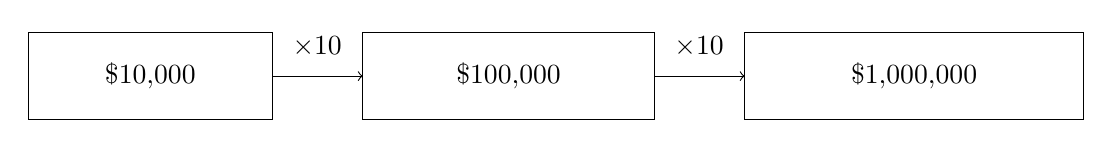
\begin{tikzpicture}
\draw (0,0) rectangle (3.1,1.1);
\node at (1.55,0.55) {\(\$10{,}000\)};

\draw (4.25,0) rectangle (7.95,1.1);
\node at (6.1,0.55) {\(\$100{,}000\)};

\draw (9.1,0) rectangle (13.4,1.1);
\node at (11.25,0.55) {\(\$1{,}000{,}000\)};

\draw[->] (3.1,0.55) -- (4.25,0.55);
\node at (3.67,0.92) {\(\times 10\)};

\draw[->] (7.95,0.55) -- (9.1,0.55);
\node at (8.52,0.92) {\(\times 10\)};
\end{tikzpicture}
\caption{The million-dollar target decomposed into repeatable units.}
\end{figure}

This is the lecture's main calming device. The million is not denied; it is factorized. Once the number is factorized, the discussion immediately returns to execution. Victor says that he did not use ad spend or a formal budget to propel the work. Instead he emphasizes bootstrapping, daily presence, and showing up regardless of the opponent or circumstance. This is a crucial motivational beat. Decomposition alone does not create revenue. Decomposition tells us what must be repeated; consistency tells us how the repetition is actually completed.

\section{Sales as Positioning}

The interviewer now pivots with real force: if scale is a game of numbers, then one bottleneck remains obvious. How do we convert a prospective client who is leaning toward no? The lecture answers this by refusing the usual psychology of the close.

\subsection{Question \& Answer}

\paragraph{Question.}
If a client or customer is on the fence and leaning toward refusal, what move turns a likely no into a yes?

\paragraph{Answer.}
Victor's first answer is entirely negative: do not push. Pressure sends the wrong signal. It makes the other side feel that we need the deal more than they need the offer. If \(P_{\text{push}}\) denotes sales pressure, then the lecture's directional claim is
\begin{equation}
P_{\text{push}} \uparrow \;\Rightarrow\; \Pr(\text{resistance}) \uparrow.
\end{equation}

The positive doctrine is a reversal of geometry. Rather than pushing harder, one tries to become so established, so attractive, and so selective that people come inward. In a compact transcript-based shorthand,
\begin{equation}
\text{quality} + \text{scale} + \text{scarcity} \;\Rightarrow\; \text{inbound demand}.
\end{equation}

We may summarize the contrast by the following schematic:

\begin{figure}
\centering
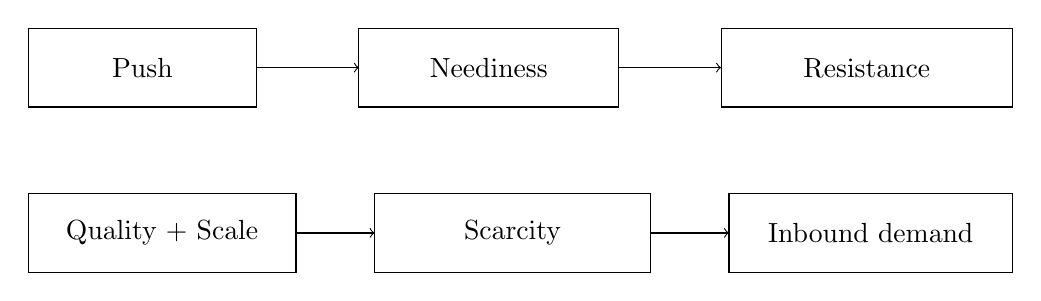
\begin{tikzpicture}
\draw (0,2.1) rectangle (2.9,3.1);
\node at (1.45,2.6) {Push};

\draw (4.2,2.1) rectangle (7.5,3.1);
\node at (5.85,2.6) {Neediness};

\draw (8.8,2.1) rectangle (12.5,3.1);
\node at (10.65,2.6) {Resistance};

\draw[->] (2.9,2.6) -- (4.2,2.6);
\draw[->] (7.5,2.6) -- (8.8,2.6);

\draw (0,0) rectangle (3.4,1.0);
\node at (1.7,0.5) {Quality + Scale};

\draw (4.4,0) rectangle (7.9,1.0);
\node at (6.15,0.5) {Scarcity};

\draw (8.9,0) rectangle (12.5,1.0);
\node at (10.7,0.5) {Inbound demand};

\draw[->] (3.4,0.5) -- (4.4,0.5);
\draw[->] (7.9,0.5) -- (8.9,0.5);
\end{tikzpicture}
\caption{The lecture's sales contrast: pressure generates resistance, while quality and scarcity generate pull.}
\end{figure}

The interview does not leave this at the level of posture. It gives a business mechanism: an elite program and a paid subscription that allowed customers onto the website earlier than everybody else. Scarcity, then, is not only emotional. It can be operationalized as tiered access. The key is that selectivity is not faked after the fact; it is built into the structure of the offer.

\section{Network as Environmental Leverage}

From sales the lecture widens once again. The next question is about relationships, but the answer is not sentimental. Victor says that, besides consistency, network is one of the most important things because one is a product of one's environment. We should hear this carefully. The claim is not that successful friends are morally elevating. The claim is that they alter the scale at which our own effort is judged.

\paragraph{Claim.}
A stronger room raises the working ceiling; a weaker room lowers it.

\paragraph{Mechanism.}
The comparison class determines what feels ordinary. If everyone around us is doing more than we are doing, then our own present scale does not feel final. If everyone around us is doing less, then we may mistake an early waypoint for an ending point.

This is why the lecture places network immediately after sales. Once we stop thinking transaction by transaction, we are forced to ask what sort of environment keeps the ambition expanding.

\subsection{Question \& Answer}

\paragraph{Question.}
Suppose we accept that the right room matters. How do we gain entry if we do not yet belong to that room and do not wish to enter with a handout?

\paragraph{Answer.}
Victor's answer is one of the cleanest in the lecture: invest in yourself until you can enter with an offer. Let \(S_{\text{offer}}\) denote the strength of the concrete value we can bring. Then the lecture suggests
\begin{equation}
S_{\text{offer}} \uparrow \;\Rightarrow\; \Pr(\text{access}) \uparrow.
\end{equation}

The transcript gives us an image for this: a puzzle piece. Someone else may have more money and more success, but if we possess a sharpened skill that fills a genuine gap, then we are no longer arriving as a petitioner. We are arriving as a complement.

The sequence is worth writing down explicitly:
\begin{enumerate}
\item Invest in the self before seeking admission.
\item Sharpen one skill until it becomes concrete and legible.
\item Find the missing piece in another person's business.
\item Offer that missing piece rather than asking vague favors.
\item Turn access into exchange.
\end{enumerate}

This argument prepares the move into finance. Once access and opportunity are cast as exchange, the next natural question is what to do with the money and time thereby unlocked.

\section{Income, Time, and the Restart from Zero}

The lecture now enters a rapid but coherent endgame. The interviewer asks, in succession, about financial advice, mindset, the most important skill, and the problem of starting over. The answers belong together because they form one operating doctrine.

First comes the financial maxim Victor attributes to Chris Johnson: get money by income. The phrase is colloquial, but the mechanism is exact enough. Income should be used to purchase assets that generate more income. If \(I\) is present income, \(A\) the acquired asset, and \(I'\) the later income stream, then the cycle is
\begin{equation}
I \to A \to I', \qquad I' > I.
\end{equation}

\begin{figure}
\centering
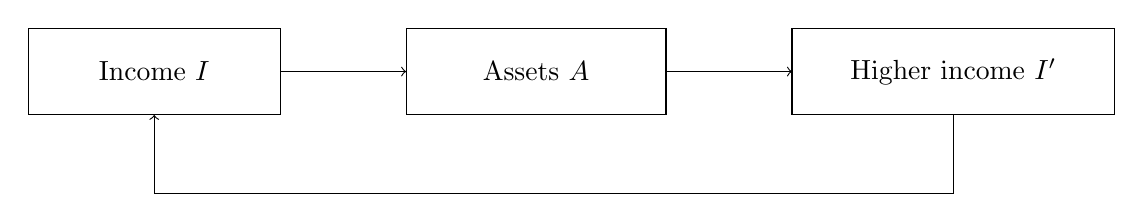
\begin{tikzpicture}
\draw (0,0) rectangle (3.2,1.1);
\node at (1.6,0.55) {Income \(I\)};

\draw (4.8,0) rectangle (8.1,1.1);
\node at (6.45,0.55) {Assets \(A\)};

\draw (9.7,0) rectangle (13.8,1.1);
\node at (11.75,0.55) {Higher income \(I'\)};

\draw[->] (3.2,0.55) -- (4.8,0.55);
\draw[->] (8.1,0.55) -- (9.7,0.55);
\draw[->] (11.75,0) -- (11.75,-1.0) -- (1.6,-1.0) -- (1.6,0);
\end{tikzpicture}
\caption{Reinvestment as a loop rather than a one-time event.}
\end{figure}

The next principle is about priority rather than cash flow. Victor says time is worth more than money. We should read this as an ordering relation, not as an exchange rate:
\begin{equation}
\text{time} \succ \text{money}.
\end{equation}
Here \(\succ\) means strategic priority. Wealth depends less on admiring the importance of time than on selecting what time is actually spent on. The lecture's contrast is memorable: attractive, easy, entertaining tasks on one side; boring, consistent, simple work on the other. Victor's claim is that the latter is what carries one to the next level.

The interview then asks for the single most important skill for a young entrepreneur. Victor answers: social media marketing. This does not arrive out of nowhere. It completes the earlier argument about attention. If the first bottleneck is visibility, then the skill that manages visibility becomes a general catalyst.

Finally, the interviewer applies a zero-reset test. Suppose the bank account returns to zero tomorrow. What is the first move? Victor's answer is procedural rather than dramatic. He says he would rely on a strong network, borrow ten thousand dollars, start a quick cash-flow business such as car detailing, stack funds, and then move back toward higher-leverage digital business.

We may record the stated seed condition as
\begin{equation}
I_0 = \$10{,}000
\end{equation}
for the restart scenario, and then write the playbook as
\begin{enumerate}
\item secure small initial capital through network trust;
\item start a fast service business to produce cash flow;
\item accumulate funds rather than waiting for an ideal grand opportunity;
\item return to more scalable digital business after liquidity has been restored.
\end{enumerate}

This is one of the lecture's deepest moments. The system is valuable not because it once produced a good outcome, but because it can be run again. The true asset is not a particular business form. It is the repeatable sequence of network, cash flow, reinvestment, and renewed scale.

The closing question asks how Victor wants to be remembered. He answers that he wants a wider reach and wants to help other people change their financial life through business and entrepreneurship. The lecture therefore ends where many serious lectures end: not with a final formula, but with a direction of use. The method is meant to travel outward.

\section{Summary}

The chapter may now be compressed without being flattened. First, the lecture turns large wealth targets into manageable units:
\[
T = u \cdot n.
\]
Second, it explains why repeated output matters in a distracted market:
\[
f_{\text{drop}} \uparrow \Rightarrow E \uparrow.
\]
Third, it replaces push-based sales with quality, selectivity, and scarcity:
\[
P_{\text{push}} \uparrow \Rightarrow \Pr(\text{resistance}) \uparrow.
\]
Fourth, it treats network as an environmental lever rather than a social ornament:
\[
S_{\text{offer}} \uparrow \Rightarrow \Pr(\text{access}) \uparrow.
\]
Fifth, it closes the loop by turning income into future income:
\[
I \to A \to I', \qquad I' > I.
\]

What begins as a success profile thus becomes a disciplined sequence. We decompose the number, we keep appearing, we refuse needy sales geometry, we enter stronger rooms by bringing value, and we cycle money back into more money. That is the lecture's arithmetic of entrepreneurial scale.